\documentclass[12pt]{article}

\usepackage{algorithmic}
\usepackage{amsmath}
\usepackage{graphicx}
\usepackage{hyperref}
\usepackage{booktabs}

\providecommand{\e}[1]{\ensuremath{\times 10^{#1}}}

\begin{document}

\title{CSI709 Homework 5 \\
Fractional Power Filter}
\author{
        Geoffrey Ulman \\
        George Mason University\\
}
\date{\today}

\maketitle

\section{Results}

Figures \ref{boats1}, \ref{boats2}, and \ref{boats3} provide samples of the cutout boat images which were used to construct the final fractional power filter.

The remaining series of images demonstrates the results of correlating the original image against the filter for various \(\alpha\) values. For each \(\alpha\) value, a peak detection image along with the threshold used, is provided. Results appear best for \(\alpha\) values around \(0.7\). Closer to \(2.0\)

\begin{figure}
\centering
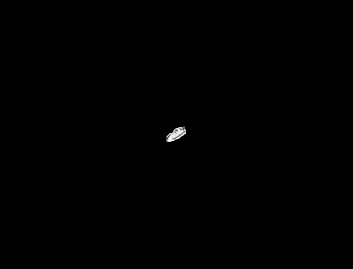
\includegraphics[width=0.50\textwidth]{plotBoat1.png}
\caption{Sample Boat Training Image 1}
\label{boats1}
\end{figure}

\begin{figure}
\centering
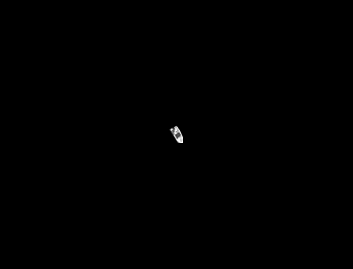
\includegraphics[width=0.50\textwidth]{plotBoat2.png}
\caption{Sample Boat Training Image 2}
\label{boats2}
\end{figure}

\begin{figure}
\centering
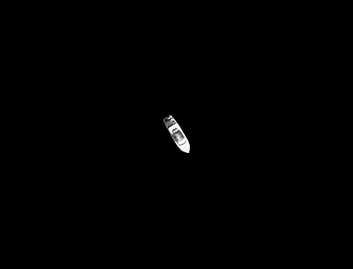
\includegraphics[width=0.50\textwidth]{plotBoat3.png}
\caption{Sample Boat Training Image 3}
\label{boats3}
\end{figure}

\begin{figure}
\centering
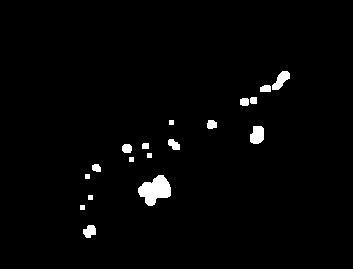
\includegraphics[width=0.80\textwidth]{v2/boats_a00_peak.png}
\caption{\(\alpha=0\) filtered peaks \(> 1.2\)}
\label{a00peak}
\end{figure}

\begin{figure}
\centering
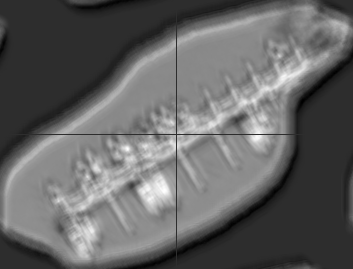
\includegraphics[width=0.80\textwidth]{v2/boats_a00.png}
\caption{\(\alpha=0\)}
\label{a00}
\end{figure}

\begin{figure}
\centering
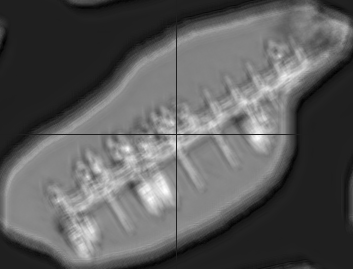
\includegraphics[width=0.80\textwidth]{v2/boats_a04_peak.png}
\caption{\(\alpha=0.4\) filtered peaks \(> 1.2\e{-5}\)}
\label{a04peak}
\end{figure}

\begin{figure}
\centering
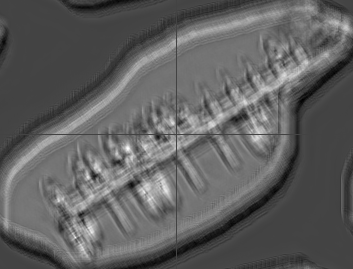
\includegraphics[width=0.80\textwidth]{v2/boats_a04.png}
\caption{\(\alpha=0.4\)}
\label{a04}
\end{figure}

\begin{figure}
\centering
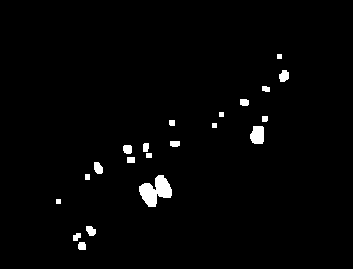
\includegraphics[width=0.80\textwidth]{v2/boats_a08_peak.png}
\caption{\(\alpha=0.8\) filtered peaks \(> 1.0\e{-5}\)}
\label{a08peak}
\end{figure}

\begin{figure}
\centering
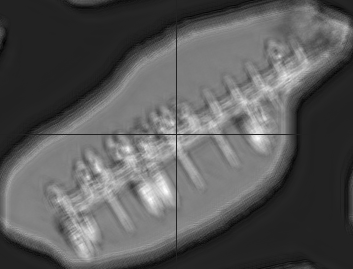
\includegraphics[width=0.80\textwidth]{v2/boats_a08.png}
\caption{\(\alpha=0.8\)}
\label{a08}
\end{figure}

\begin{figure}
\centering
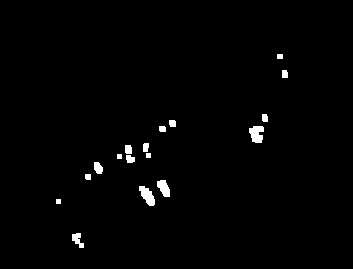
\includegraphics[width=0.80\textwidth]{v2/boats_a12_peak.png}
\caption{\(\alpha=1.2\) filtered peaks \(> 7.5\e{-6}\)}
\label{a12peak}
\end{figure}

\begin{figure}
\centering
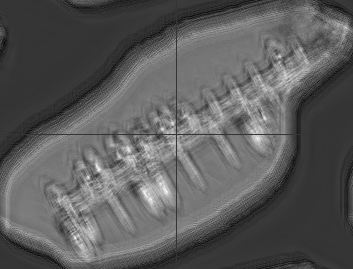
\includegraphics[width=0.80\textwidth]{v2/boats_a12.png}
\caption{\(\alpha=1.2\)}
\label{a12}
\end{figure}

\begin{figure}
\centering
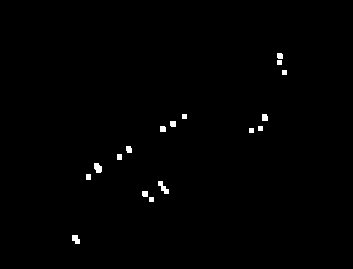
\includegraphics[width=0.80\textwidth]{v2/boats_a16_peak.png}
\caption{\(\alpha=1.6\) filtered peaks \(> 6.0\e{-6}\)}
\label{a16peak}
\end{figure}

\begin{figure}
\centering
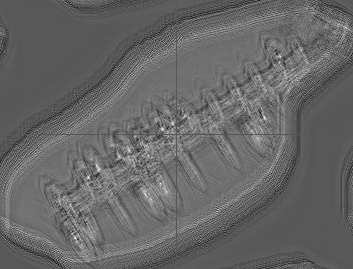
\includegraphics[width=0.80\textwidth]{v2/boats_a16.png}
\caption{\(\alpha=1.6\)}
\label{a16}
\end{figure}

\begin{figure}
\centering
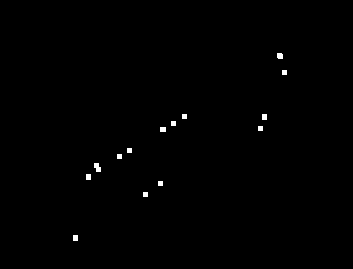
\includegraphics[width=0.80\textwidth]{v2/boats_a20_peak.png}
\caption{\(\alpha=2.0\) filtered peaks \(> 6.0\e{-6}\)}
\label{a20peak}
\end{figure}

\begin{figure}
\centering
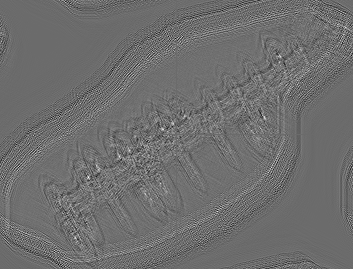
\includegraphics[width=0.80\textwidth]{v2/boats_a20.png}
\caption{\(\alpha=2.0\)}
\label{a20}
\end{figure}

\begin{figure}
\centering
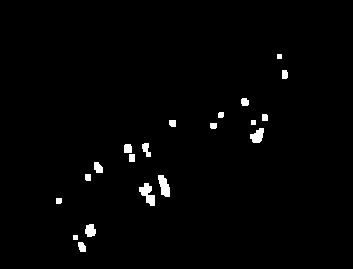
\includegraphics[width=0.80\textwidth]{v2/boats_a08_missing_peak.png}
\caption{\(\alpha=0.8\) filtered peaks \(> 1.0\e{-5}\) trained against boat 16, 17}
\label{a07missingpeak}
\end{figure}

\begin{figure}
\centering
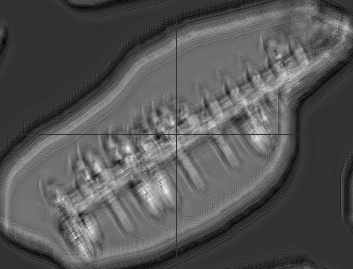
\includegraphics[width=0.80\textwidth]{v2/boats_a08_missing.png}
\caption{\(\alpha=0.8\) trained against boat 16, 17}
\label{a07missing}
\end{figure}

\end{document}
